\documentclass[xcolor=dvipsnames,10pt]{beamer}
\usepackage[utf8]{inputenc}
\usepackage[T1]{fontenc}
\usepackage[brazilian]{babel}
\usepackage{etoolbox}
\usepackage{graphicx}
\usepackage{ragged2e}
\usepackage{tikz}
\usepackage{subfig}
\usepackage{graphics}


\makeatletter
\patchcmd{\beamer@sectionintoc}{\vskip1.5em}{\vskip0.5em}{}{}
\makeatother

\usefonttheme[professional]{serif}

\justifying

%----------------------------------------------------------------------------------------------------------------------------------

% JUSTIFICAR TEXTO DAS LISTAS DE ITENS

\makeatletter
\renewcommand{\itemize}[1][]{%
  \beamer@ifempty{#1}{}{\def\beamer@defaultospec{#1}}%
  \ifnum \@itemdepth >2\relax\@toodeep\else
    \advance\@itemdepth\@ne
    \beamer@computepref\@itemdepth% sets \beameritemnestingprefix
    \usebeamerfont{itemize/enumerate \beameritemnestingprefix body}%
    \usebeamercolor[fg]{itemize/enumerate \beameritemnestingprefix body}%
    \usebeamertemplate{itemize/enumerate \beameritemnestingprefix body begin}%
    \list
      {\usebeamertemplate{itemize \beameritemnestingprefix item}}
      {\def\makelabel##1{%
          {%
            \hss\llap{{%
                \usebeamerfont*{itemize \beameritemnestingprefix item}%
                \usebeamercolor[fg]{itemize \beameritemnestingprefix item}##1}}%
          }%
        }%
      }
  \fi%
  \beamer@cramped%
  \justifying% NEW
  %\raggedright% ORIGINAL
  \beamer@firstlineitemizeunskip%
}
\makeatother

%%%%%%%%%%%%%%%%%%%%%%%%%%%%

%%%%%%%%%%%%%%%%%%%%%%%%%%%%%%%%%%%%%%%%%%%%%%%%%%%%%%%%%%%%%%%%%%%%%%%%%%%%%%%%
%COR DO TEMPLATE SEMELHANTE AO LOGO
%%%%%%%%%%%%%%%%%%%%%%%%%%%%%%%%%%%%%%%%%%%%%%%%%%%%%%%%%%%%%%%%%%%%%%%%%%%%%%%%
\definecolor{azul}{rgb}{0.16, 0.32, 0.75}

%%%%%%%%%%%%%%%%%%%%%%%%%%%%%%%%%%%%%%%%%%%%%%%%%%%%%%%%%%%%%%%%%%%%%%%%%%%%%%%%
%CORES E ESTRUTURAS DE ELEMENTOS DIVERSOS
%%%%%%%%%%%%%%%%%%%%%%%%%%%%%%%%%%%%%%%%%%%%%%%%%%%%%%%%%%%%%%%%%%%%%%%%%%%%%%%%
\setbeamercolor{frametitle}{fg=black}
\setbeamercolor{headline}{fg=black}
\setbeamercolor{footline}{fg=black}
\setbeamercolor{block body}{use=structure,bg=white}
\setbeamercolor{block title}{use=structure,bg=azul,fg=black}
\setbeamercolor{item}{fg=azul}
\setbeamercolor{alerted text}{fg=azul}
\setbeamercolor{section in toc}{fg=black}
\setbeamercolor{title}{fg=black}
\setbeamercolor{subtitle}{fg=black}
\setbeamertemplate{blocks}[rounded][shadow=true]

%%%%%%%%%%%%%%%%%%%%%%%%%%%%%%%%%%%%%%%%%%%%%%%%%%%%%%%%%%%%%%%%%%%%%%%%%%%%%%%%
%PROPRIEDADES VISUAIS DE ELEMENTOS DIVERSOS
%%%%%%%%%%%%%%%%%%%%%%%%%%%%%%%%%%%%%%%%%%%%%%%%%%%%%%%%%%%%%%%%%%%%%%%%%%%%%%%%
\useoutertheme[]{default}
\addtobeamertemplate{block begin}{}{\justifying} % Justify all blocks

\setbeamertemplate{section in toc}[circle]
\setbeamertemplate{subsection in toc}[square]
\setbeamertemplate{itemize item}{$\bullet$}
\setbeamertemplate{navigation symbols}{}
\setbeamercovered{invisible}
\setbeamertemplate{sections in toc}[ball]


%%%%%%%%%%%%%%%%%%%%%%%%%%%%%%%%%%%%%%%%%%%%%%%%%%%%%%%%%%%%%%%%%%%%%%%%%%%%%%%%
%LOGO DO EVENTO COMO TÍTULO DE TODOS OS SLIDES
%%%%%%%%%%%%%%%%%%%%%%%%%%%%%%%%%%%%%%%%%%%%%%%%%%%%%%%%%%%%%%%%%%%%%%%%%%%%%%%%
\setbeamertemplate{headline}{

\vspace{-1em}
\begin{center}

\includegraphics[width=0.7\textwidth]{logo.jpg}
\end{center}
}

%%%%%%%%%%%%%%%%%%%%%%%%%%%%%%%%%%%%%%%%%%%%%%%%%%%%%%%%%%%%%%%%%%%%%%%%%%%%%%%%
% INICIO DOS SLIDES
%%%%%%%%%%%%%%%%%%%%%%%%%%%%%%%%%%%%%%%%%%%%%%%%%%%%%%%%%%%%%%%%%%%%%%%%%%%%%%%%

\title{\textsc{INDICADOR INDIRETO DE ROTAÇÃO EM AGLOMERADOS DE GALÁXIAS}}
\author{
  \textbf{Autor} \\
  Luenne Nailam Sousa Nascimento \\
  \textbf{Orientador} \\
  Prof. Dr. André Luis Batista Ribeiro
}

\begin{document}

\frame{\titlepage}
\frame{\tableofcontents}
\section{Introdução}

\subsection{Aglomerados de Galáxias}

\begin{frame}{\textbf{Aglomerado de Galáxias}}
\begin{itemize}
\item Aglomerados de galáxias são as maiores estruturas do Universo observável que podem ter alcançado o estado em equilíbrio dinâmico.
\item Aglomerados de galáxias são definidos basicamente por três componentes: galáxias, meio intra-aglomerado e matéria escura.
\end{itemize}
 \begin{figure}[!htbp] %h or !htbp
    \begin{center}
    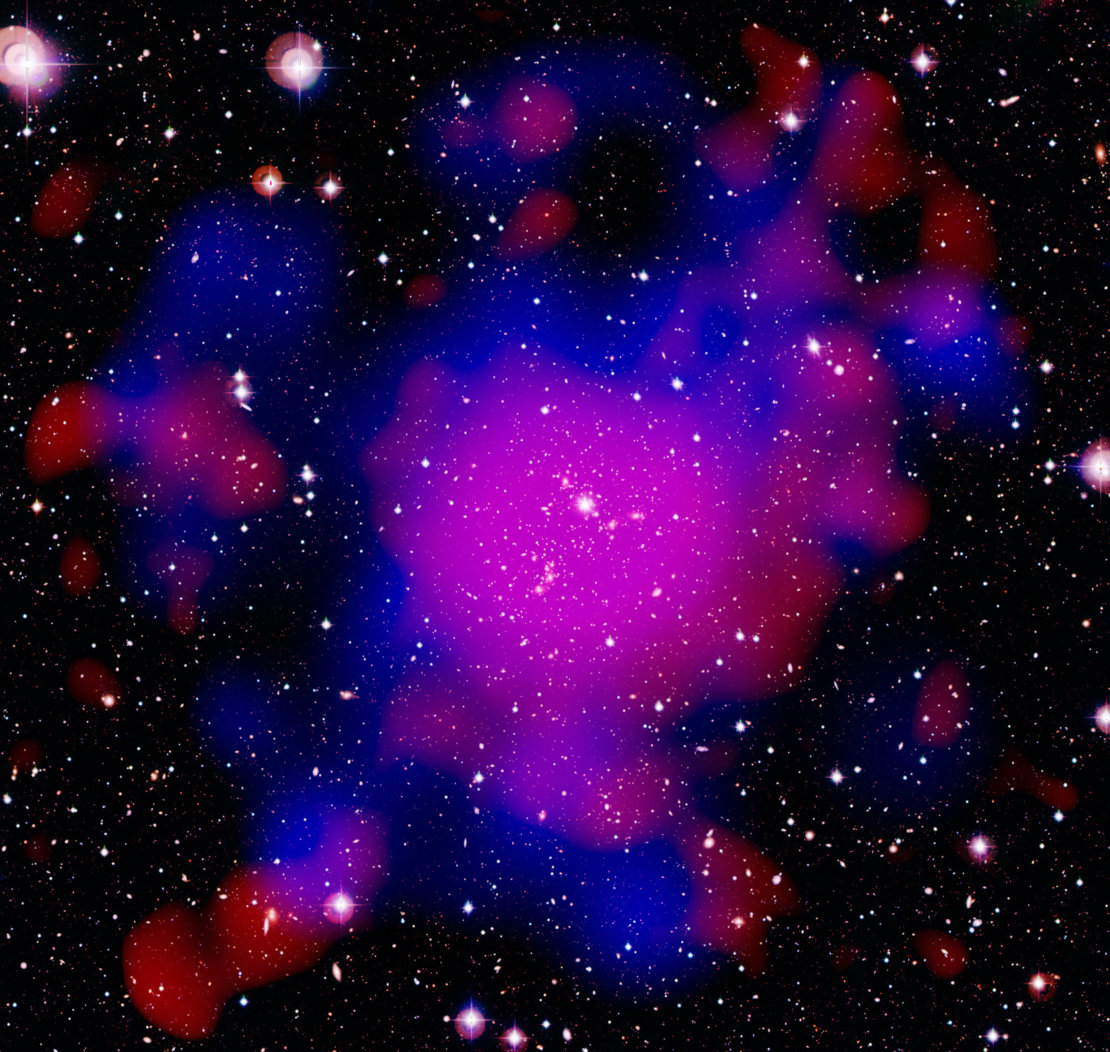
\includegraphics[height=0.5\textheight,width=0.7\textwidth]{resultados/cluster.jpg}%
    \caption{\scriptsize{Composição de um Aglomerado.}}
    \end{center}
  \end{figure} 
\end{frame}

\begin{frame}{\textbf{Aglomerado de Galáxias}}
\begin{itemize}
	\item A busca por compreender a formação e evolução dos aglomerados de galáxias é uma das questões mais importantes da Astrofísica. 
	\item  No paradigma atual de formação das estruturas, as galáxias e os aglomerados surgem a partir de halos escuros.
	\begin{itemize}
	\item Aglomerados formados após as galáxias em um desvio para o vermelho $z \approx 2$.
	\end{itemize}
\end{itemize}
\end{frame}

\begin{frame}{\textbf{Aglomerado de Galáxias}}
 \begin{figure}[!htbp] %h or !htbp
    \begin{center}
    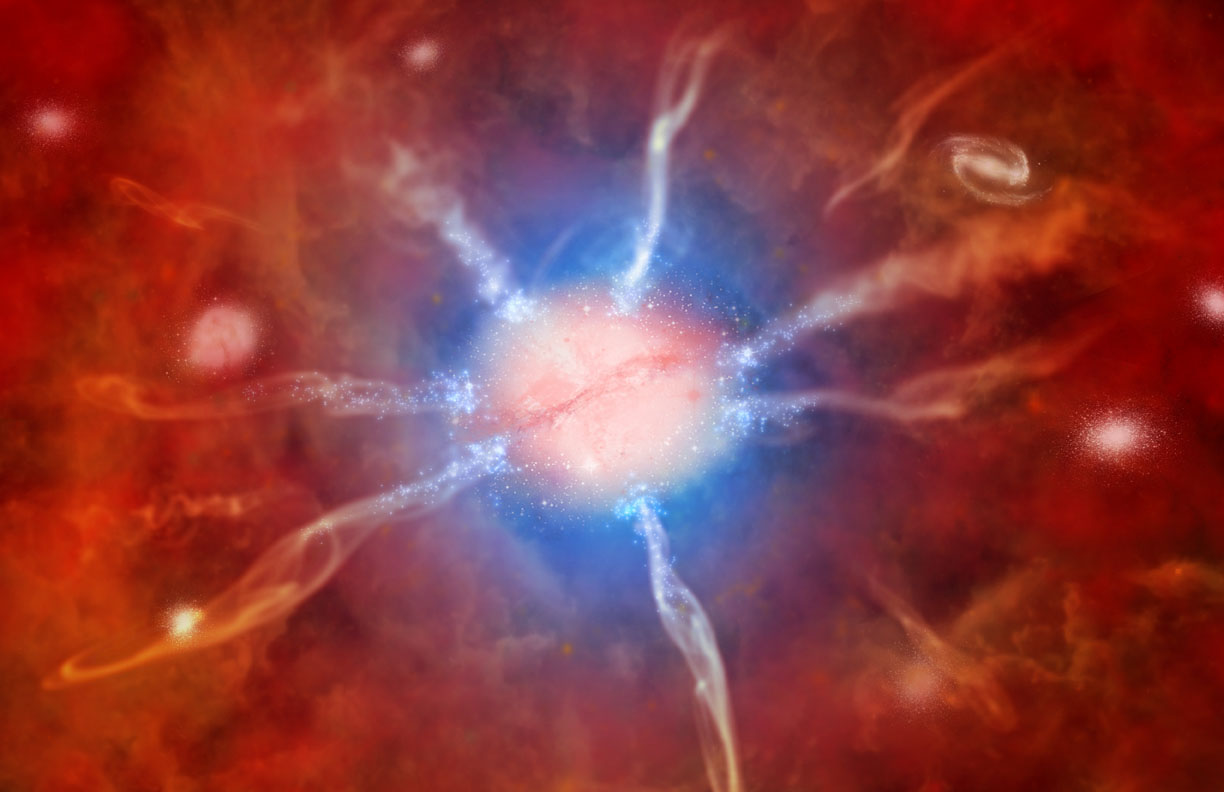
\includegraphics[height=0.5\textheight,width=0.7\textwidth]{resultados/formation.jpg}%
    \caption{\scriptsize{Aglomerado em processo de interação com galáxias ou grupo de galáxias.}}
    \end{center}
  \end{figure} 
\end{frame}

\begin{frame}{\textbf{Aglomerado de Galáxias}}
\begin{itemize}
\item O processo de formação de aglomerados não atingiu seu fim.
\begin{itemize}
\item Distribuição de velocidades é bem ajustada por uma gaussiana somente na região virializada do sistema. Enquanto a periferia do sistema é continuamente perturbada por acréscimo de matéria.
\end{itemize}
\end{itemize}
\end{frame}

\begin{frame}{\textbf{Aglomerado de Galáxias}}
\begin{figure}[!htbp] %h or !htbp
\begin{center}
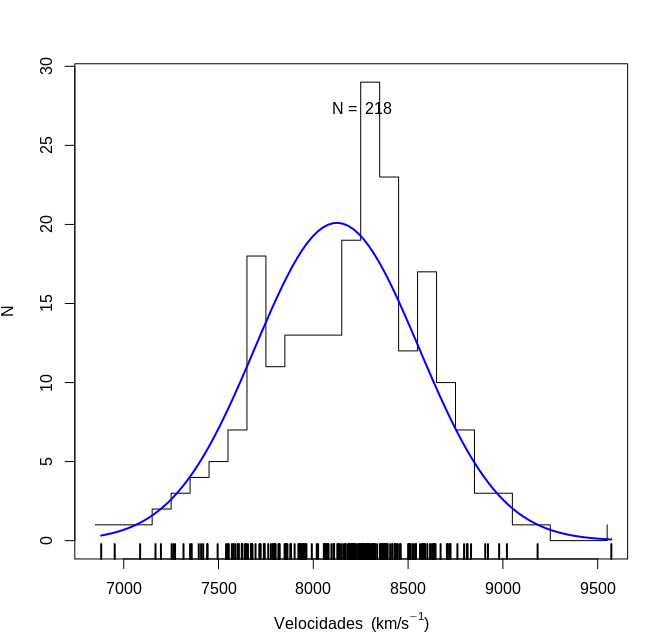
\includegraphics[height=0.6\textheight,width=0.7\textwidth]{10043dist}%
\caption{\scriptsize{Histograma de velocidades de um dos aglomerados de nossa amostra.}}
\label{fig1}%
\end{center}
\end{figure}  
\end{frame}

\subsection{Distribuição de Velocidades ao longo do Aglomerado}
\begin{frame}{\textbf{Distribuição de Velocidades ao longo do Aglomerado}}
\begin{itemize}
\item A velocidade de uma galáxia contida em um aglomerado, em uma dada posição, não pode ser maior que a velocidade de escape do sistema.
\item A velocidade de escape e a distância ao centro do aglomerado são grandezas inversamente proporcionais. 
\item O  perfil radial da velocidade de escape permite definir os galáxias membro dos aglomerados.
\end{itemize} 
\end{frame}

\begin{frame}{\textbf{Distribuição de Velocidades ao longo do Aglomerado}}
  \begin{figure}[!htbp] %h or !htbp
    \begin{center}
    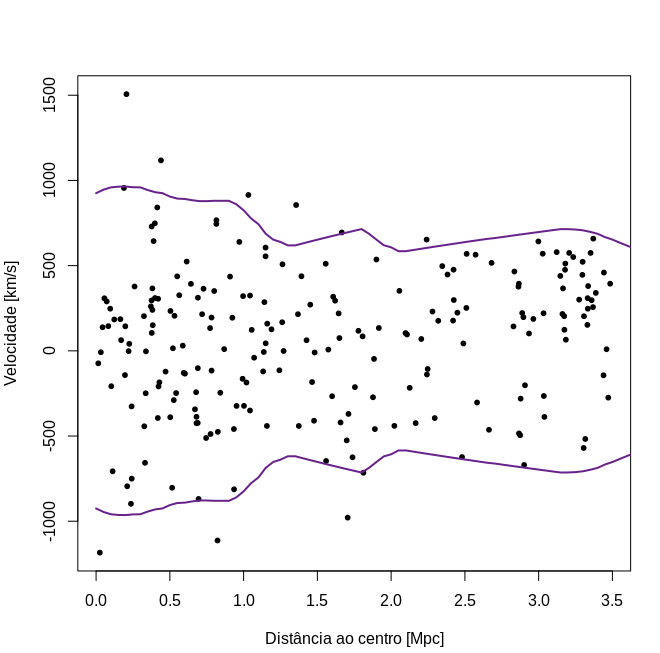
\includegraphics[height=0.6\textheight,width=0.7\textwidth]{10043}%
    \caption{\scriptsize{Distribuição de velocidades em função da distância ao centro de um dos aglomerados de nossa amostra.}}
    \label{fig1}%
    \end{center}
  \end{figure} 
\end{frame}

\begin{frame}
  \begin{itemize}
    \item Após a determinação dos membros de um aglomerado, suas propriedades dinâmicas, como massa e raio, podem ser estimadas.
    \begin{itemize}
      \item O método mais empregado é o de análise do virial.
    \end{itemize} 
  \end{itemize}
  \begin{figure}[!htbp] %h or !htbp
    \begin{center}
    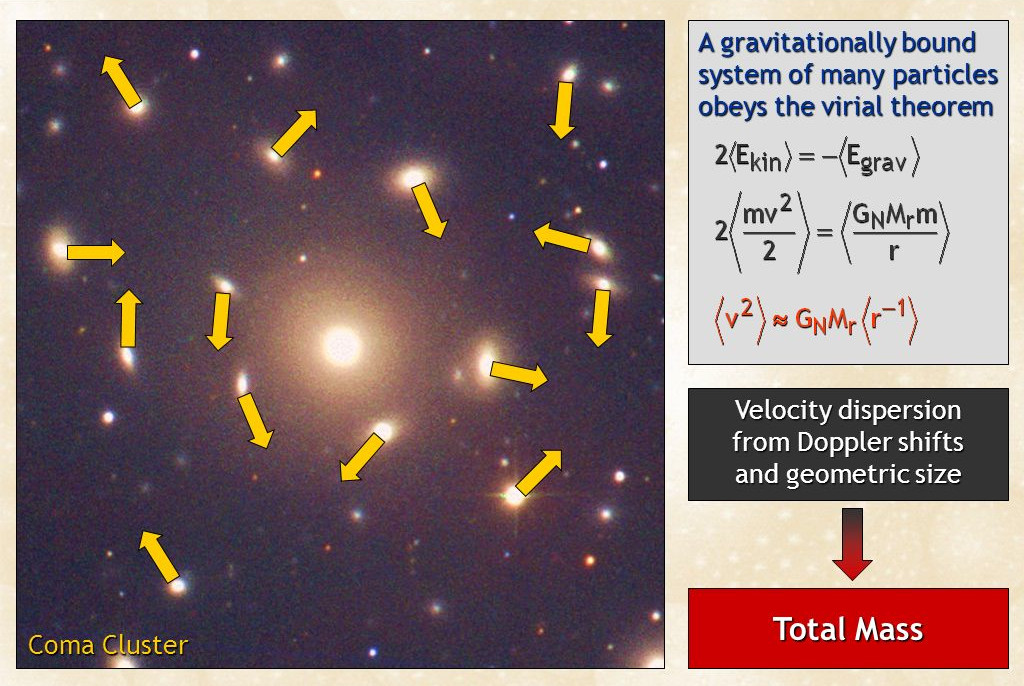
\includegraphics[height=0.5\textheight,width=0.7\textwidth]{resultados/virial.jpg}%
    \caption{\scriptsize{Análise do virial utiliza apenas as velocidades aleatórias das galáxias na região central do aglomerado.}}
    \end{center}
  \end{figure} 
\end{frame}

\subsection{Rotação de Aglomerados}
\begin{frame}{\textbf{Rotação de Aglomerados}}
\begin{itemize}
  \item {\textbf{Hwang \& Lee (2007):}}  
  \begin{itemize}
    \item \textbf{Amostra:} Dados espectroscópicos do Sloan Digital Sky Survey (SDSS) e Two-Degree-Field Galaxy Redshift Survey (2dF-GRS).
    \item \textbf{Objetivo:} A busca por aglomerados de galáxias que mostrem uma indicação de rotação global.
    \item \textbf{Conclusão e Resultados:}
    \begin{itemize}
      \item Foram detectados seis sistemas com rotação, em um total de doze aglomerados.
      \item Os aglomerados com rotação devem exibir divisão espacial entre galáxias com velocidades maiores e menores que a velocidade média do aglomerado além de apresentar um pico no mapa de densidade.
      \item Constatou-se ainda que estes aglomerados estão em equilíbrio dinâmico e não sofreram fusão recente.
    \end{itemize}
  \end{itemize}
\end{itemize}
\end{frame}

\begin{frame}{\textbf{Rotação de Aglomerados}}
\begin{itemize}
  \item {\textbf{Kalinkov et al. (2008):}}  
    \begin{itemize}
      \item \textbf{Amostra:} Aglomerado de Abell 2107.
      \item \textbf{Objetivo:} Identificar a rotação do aglomerado de galáxias A2107.
      \item \textbf{Conclusão e Resultados:}
      \begin{itemize}
        \item O método buscou o gradiente máximo no campo de velocidade e determinou que a direção do coeficiente de correlação linear máximo definiria o eixo maior do aglomerado e o eixo menor seria o de rotação.
        \item A massa foi corrigida (inicial era de $3.2\times10^{14}~{\rm M_\odot}$ e passou para $2.8\times10^{14}~{\rm M_\odot}$).
        \item Materne et al. (1983) apontaram a dificuldade em diferenciar um aglomerado rotativo de dois que se sobrepõem, pelo motivo de estar se fundindo ou se afastando.
      \end{itemize}
    \end{itemize}
\end{itemize}
\end{frame}

\begin{frame}{\textbf{Rotação de Aglomerados}}
\begin{itemize}
  \item {\textbf{Tovmassian (2015):}}  
    \begin{itemize}
      \item \textbf{Objetivo:} Detectar a rotação de aglomerados de galáxias baseado no estudo da distribuição de velocidades das galáxias membro.
      \item \textbf{Conclusão e Resultados:}
      \begin{itemize}
        \item Constatou-se 17 aglomerados rotativos de 65.
        \item Taxa maior em aglomerados planos $f=a/b > 1.8$, (7 aglomerados rotativos em um total de 18).
        \item Os aglomerados foram originalmente formados a partir das enormes nuvens de gás primordiais e preservaram a rotação das nuvens primordiais, a menos que sofram fusões com outros aglomerados e grupos de galáxias.
      \end{itemize}
    \end{itemize}
\end{itemize}
\end{frame}

\begin{frame}{\textbf{Rotação de Aglomerados}}
\begin{itemize}
  \item {\textbf{Manolopoulou (2014):}}
    \begin{itemize}
      \item \textbf{Amostra:} Inicialmente os testes foram realizados em aglomerados gerados em simulações de Monte Carlo, posteriormente foi utilizado a amostra dos aglomerados de Abell com $z \approx 0.1$ do SDSS DR10.
      \item \textbf{Objetivo:} Identificação de rotação em aglomerados de galáxias usando a velocidade radial projetada.
      \item \textbf{Conclusão e Resultados:}
      \begin{itemize}
        \item Utilizando o teste Kolmogorov-Smirnov, decidiu-se quanto a sua rotação significativa ou não, seu centro rotacional, orientação do eixo de rotação, amplitude de velocidade rotacional e o sentido de rotação no sentido horário ou anti-horário no plano do céu.
        \item Constatou-se 23 aglomerados possivelmente rotativos dentro de 1.5 Mpc ou a uma distância de 2.5 Mpc do centro do aglomerado, de 45 da amostra.
      \end{itemize}
    \end{itemize}
\end{itemize}
\end{frame}

\begin{frame}{\textbf{Rotação de Aglomerados}}
\begin{itemize}
  \item {\textbf{Nascimento et al (2016):}}  
    \begin{itemize}
      \item \textbf{Amostra:} Par de aglomerados de Abell (A3407 e A3408) observadas no Cerro Tololo Interamerican Observatory (CTIO).
      \item \textbf{Objetivo:} Verificar se a amostra correspondia a um simples sistema de galáxias ou a um processo de fusão.
      \item \textbf{Conclusão e Resultados:}
      \begin{itemize}
        \item Ambos os sistemas bem como cada aglomerado individual tem uma distribuição de velocidade Gaussiana.
        \item Um gradiente de velocidade de $\approx 847 \pm 114\; {\rm km~s^{-1}}$ foi identificada ao redor do eixo principal da distribuição de galáxias projetada.
        \item O estudo do \textit{gap} permitiu encontrar diferença significativa entre estas subamostras.
      \end{itemize}
    \end{itemize}
\end{itemize}
\end{frame}

\section{Objetivos}
\begin{frame}{\textbf{Objetivos}}
  \begin{itemize}
    \item {\textbf{Objetivo Geral: }}
    \begin{itemize}
      \item Detecção da rotação em aglomerados para correção da sua massa.
    \end{itemize}
    \item {\textbf{Objetivos Específicos: }}
    \begin{itemize}
      \item Implementar método de detecção de rotação;
      \item Identificar a velocidade rotacional;
      \item Aplicar o Teorema do Viral para correção da massa do aglomerado.
    \end{itemize}
  \end{itemize}
\end{frame}

\section{Metologia}

\subsection{Catálogos}
\begin{frame}{\textbf{Catálogo I - selec20}}
  \begin{itemize}
    \item Um catálogo de 20 aglomerados ricos do SDSS, localizados em baixos $redshifts$, com espectroscopia disponível para objetos com $m_r \leq 17.77$.
    \item A amostra foi estudada previamente por Lopes et al. (2009) que definiu e selecionou as galáxias membro estatisticamente.
  \end{itemize}
\end{frame}

\begin{frame}{\textbf{Catálogo II - NoSOCS}}
  \begin{itemize}
    \item Um catálogo de 183 aglomerados, localizados em baixos $redshifts$ ($z \leq 0.10$), elaborado a partir da versão digitalizada do Segundo Levantamento do Observatório de Palomar.
    \item A análise foi estendida para sistemas mais ricos, incluindo os aglomerados CIRS (Cluster Infall Regions in the SDSS) Rines e Diaferio (2006), com 56 objetos.
  \end{itemize}
\end{frame}

\begin{frame}{\textbf{Catálogo III - Simulado}}
  \begin{itemize}
    \item Esferas de NFW (NAVARRO et al., 1997), ou seja, modelos simulados de sistemas esféricos com ou sem rotação
    \item O código foi desenvolvido em linguagem fortran pelo Dr. Claudio Soriano Brandão, cedido para uso neste trabalho.
  \end{itemize}
\end{frame}

\subsection{Algoritmo}
\begin{frame}{\textbf{Algoritmo}}
  \begin{enumerate}
    \item Estudo da distribuição de velocidades das galáxias membro do aglomerado em busca de gaps significativos.
    \begin{itemize}
      \item Identifica a probabilidade de que um \textit{gap}, de certo tamanho e em dada localização, possa ser reproduzido a partir de amostragens aleatórias retiradas de uma gaussiana.
      \item Consideramos \textit{gaps} com valores maiores que 2.25, uma vez que em retiradas aleatórias de uma gaussiana, \textit{gaps} desse tamanho ocorrem no máximo em 3\% dos casos (Wainer \& Shacht 1978. Beers et al. 1991).
    \end{itemize}
  \end{enumerate}
\end{frame}

\begin{frame}{\textbf{Algoritmo}}
  \begin{block}{Valor \textit{gap}}
  \begin{equation}
    g_i = v_{i+1} - v_i
  \end{equation}
  \begin{center}
  \begin{equation}
    w_i=i(N-i)
  \end{equation}
  \begin{center}
  		\hspace{10 ex} exemplo: N = 100\newline
    	\textit{para = 1} \hspace{15 ex}  \textit{para = 50}\newline
    	$w_1 = 1(99) = 99 \hspace{6 ex} w_{50} = 50(50) = 2500$
  \end{center}
  \end{center}
  \begin{equation}
    MM = \frac{2}{N} \sum_{i=N/4}^{3N/4} \sqrt{w_i g_i}
  \end{equation}
  \end{block}
\end{frame}

\begin{frame}{\textbf{Algoritmo}}
  \begin{enumerate}
    \item[2.] Os dados são divididos em duas amostras, contendo objetos com velocidades maiores e velocidades menores do que o maior \textit{gap} (\textbf{Amostras I e II}).
    \item[3.] Determina-se então o eixo principal do aglomerado como aquele resultante do ajuste de uma elipse aos dados projetados no plano do céu (pacote: \textbf{\textit{ellipse}}).
    \item[4.] As amostras I e II são então comparadas em relação a sua distribuição de duas maneiras: independente do eixo principal e em cada lado do eixo.
    \begin{itemize}
      \item Realizamos os testes de Cramér 2D e o de Hotelling.
    \end{itemize}
  \end{enumerate}
\end{frame}

\begin{frame}{\textbf{Algoritmo}}
  \begin{figure}
     \centering
    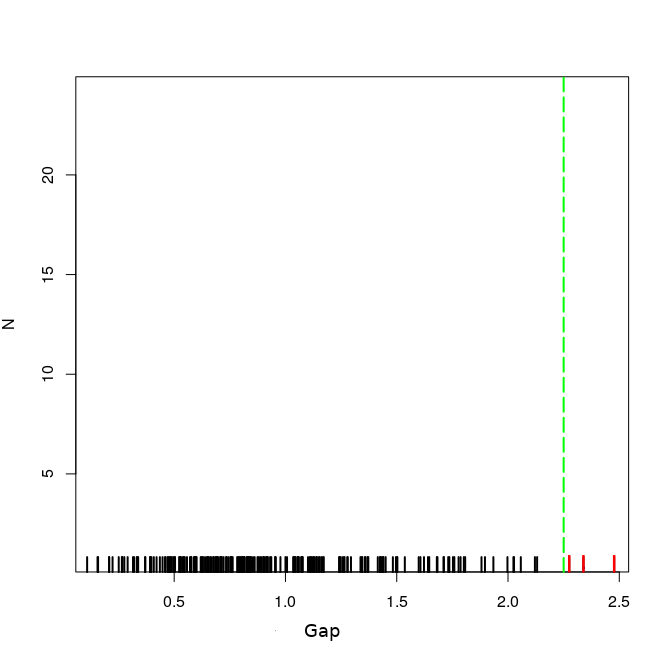
\includegraphics[height=0.7\textheight,width=0.7\textwidth]{resultados/gaps.png}
    \caption{Histograma dos gaps, em vermelho os gaps significativos do Aglomerado 01 e a linha tracejada ao ponto 2.25.}
  \end{figure}
\end{frame}

\begin{frame}{\textbf{Algoritmo}}
  \begin{block}{{\textbf{Teste de Crámer 2D}}}
    \begin{itemize}
      \item É uma medida de associação entre duas variáveis nominais dado o intervalo de 0 a 1, indicando que um valor mais alto possui forte associação.
      \begin{equation}
        \ V = \sqrt{\frac{{\chi_{obt}}^2}{N.m}}
        \label{eq:eq1}
        \end{equation}
  
        onde \textbf{$\chi^2$} é o valor obtido do teste estatístico,
        \textbf{N} é o tamanho da amostra e
        \textbf{m} = o menor de (r - 1) ou (c – 1), sendo r o número de linhas e c o número de colunas.
      \item \textbf{Hipótese nula ($H_0$)}: duas amostras não são dependentes uma da outra.
      \item \textbf{Hipótese alternativa ($H_1$)}: existe alguma associação entre duas amostras.
    \end{itemize}
  \end{block}
\end{frame}

\begin{frame}{\textbf{Algoritmo}}
  \begin{block}{{\textbf{Teste de Hotelling}}}
    \begin{itemize}
      \item  Um dos mais conhecidos testes de hipóteses multivariados, o teste de $T^2$, compara vetores de médias populacionais.
      \item Baseado na generalização da estatística \textit{t de Student}, foi o primeiro a levar em consideração a correlação das variáveis na formulação da estatística do teste.
      \begin{equation}
        H_0 : [\mu] = [\mu_0] \hspace{6 ex} H_1 : [\mu] \neq [\mu_0],     
        \end{equation}
  
        onde $[\mu_0]$ é um valor pré-especificado para a forma média.
    \end{itemize}
  \end{block}
\end{frame}

\begin{frame}{\textbf{Algoritmo}}
  \begin{enumerate}
    \item[5.] Dado que as distribuições espaciais das amostras I e II sejam distintas com 95\% de confiança em relação aos testes (passo 4), interpretamos o resultado como sendo uma indicação indireta de rotação nos aglomerados.
    \item[6.] Para os aglomerados onde isto acontece, traçamos um perfil de velocidade de rotação ao longo da distância ao centro do aglomerado.
    \item[7.] Caso o aglomerado não tenha \textit{gap} significativo (> 2.25), utilizamos a mediana dos dados como divisor das velocidades do sistema.
  \end{enumerate}
\end{frame}

\begin{frame}{\textbf{Linguagem R}}
	\begin{itemize}
		\item Linguagem que surgiu em 1993 e é considerada multi-paradigma: sequencialização, orientado a objetos, imperativo, dinâmico.
		\item Muito utilizada na manipulação, análise e visualização gráfica de dados.
		\item Pacotes utilizados:
		\begin{itemize}
			\item \textbf{\textit{ellipse}};
			\item \textbf{\textit{cramer}};
			\item \textbf{\textit{hotelling}};
			\item \textbf{\textit{astro}}.
		\end{itemize}
	\end{itemize}
\end{frame}

\begin{frame}{\textbf{Fluxograma}}
  \begin{figure}[!htbp]
    \centering
    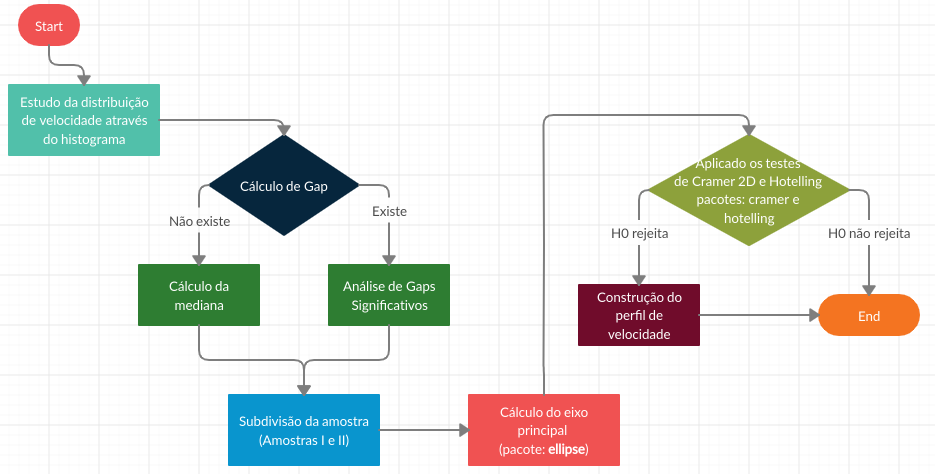
\includegraphics[scale=.4]{resultados/fluxograma.png}
  \end{figure}
\end{frame}

\section{Resultados Preliminares}
\begin{frame}{\textbf{Resultados Preliminares}}
  \begin{figure}[!htbp]
    \centering
    \subfloat{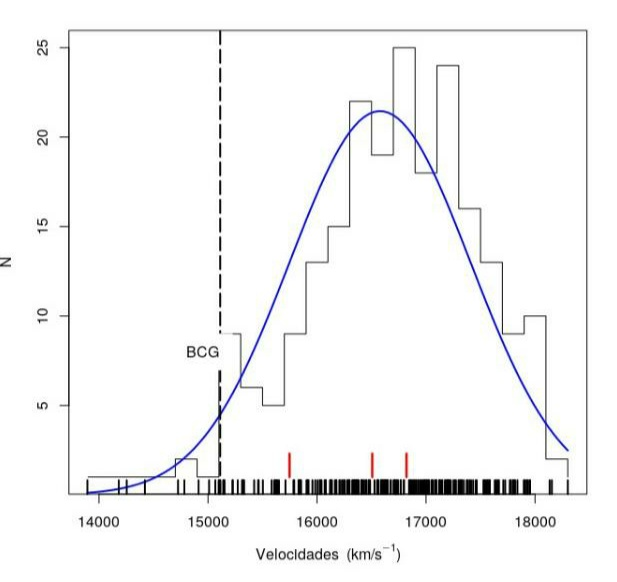
\includegraphics[scale=.23]{resultados/dist1}}
    \subfloat{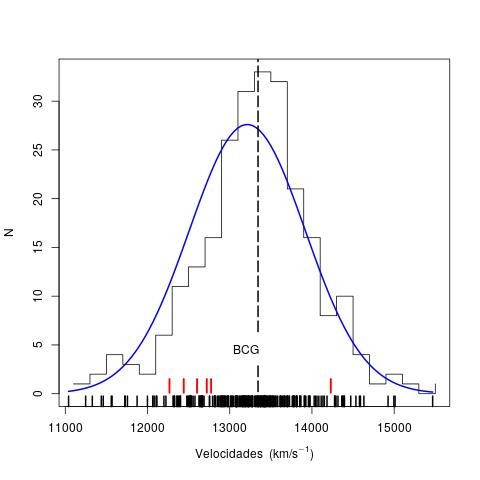
\includegraphics[scale=.3]{resultados/dist2}}
    \caption{Histograma Distribuição de Velocidade e Análise de \textit{gaps} Aglomerados 01 e 02.}
    \label{fig:fig4}%
  \end{figure}
\end{frame}

\begin{frame}{\textbf{Resultados Preliminares}}
  \begin{figure}[!htbp]
    \centering
    \subfloat{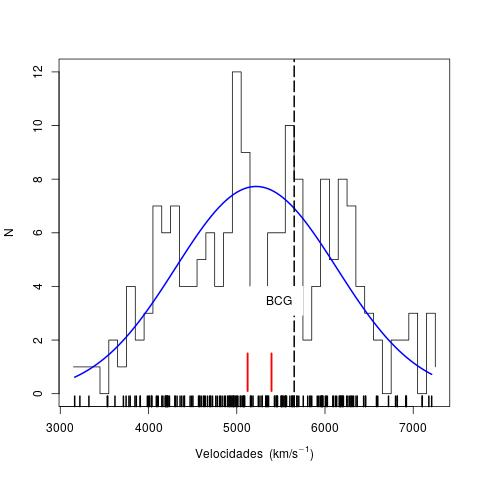
\includegraphics[scale=.23]{resultados/dist3}}
    \subfloat{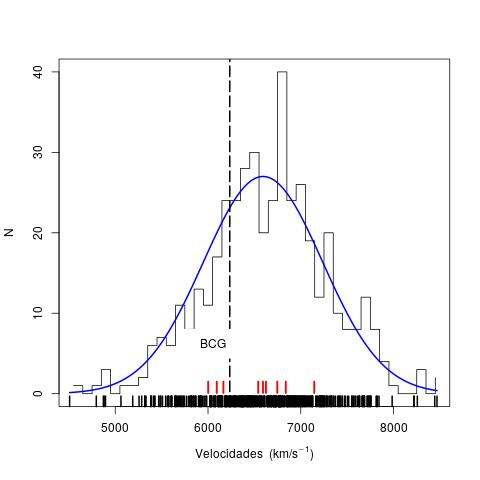
\includegraphics[scale=.23]{resultados/dist4}}
    \subfloat{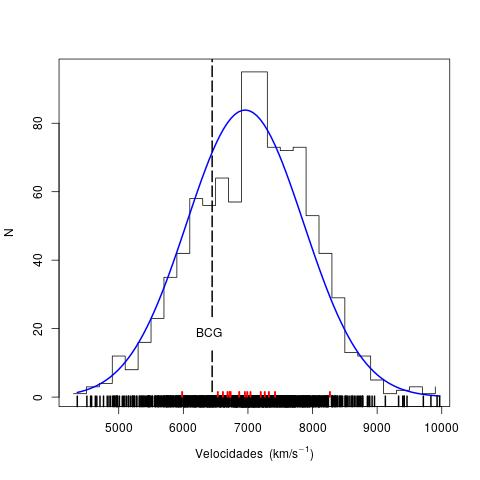
\includegraphics[scale=.23]{resultados/dist5}}
    \caption{Histograma Distribuição de Velocidade e Análise de \textit{gaps} Aglomerados 03, 04 e 05.}
  \end{figure}
\end{frame}

\begin{frame}{\textbf{Resultados Preliminares}}
  \begin{figure}[!htbp]
    \centering
    \subfloat{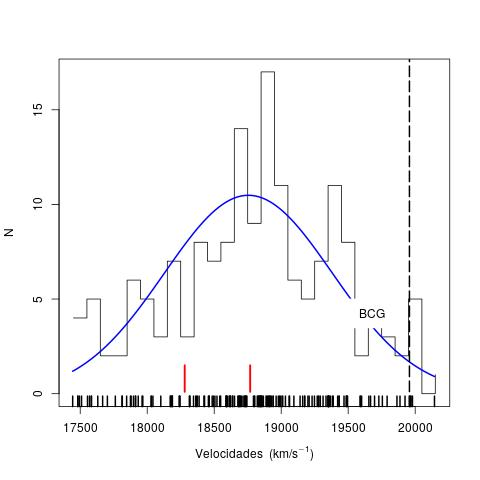
\includegraphics[scale=.23]{resultados/dist6}}
    \subfloat{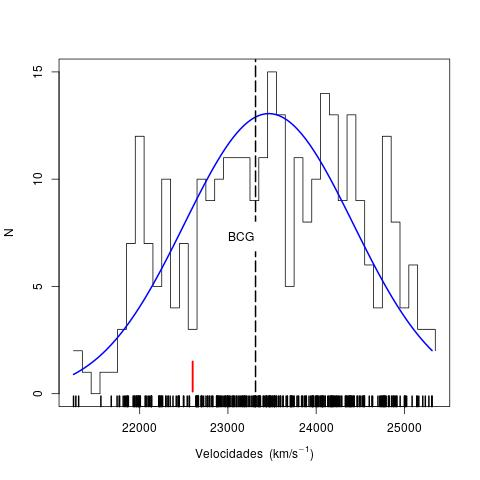
\includegraphics[scale=.23]{resultados/dist7}}
    \subfloat{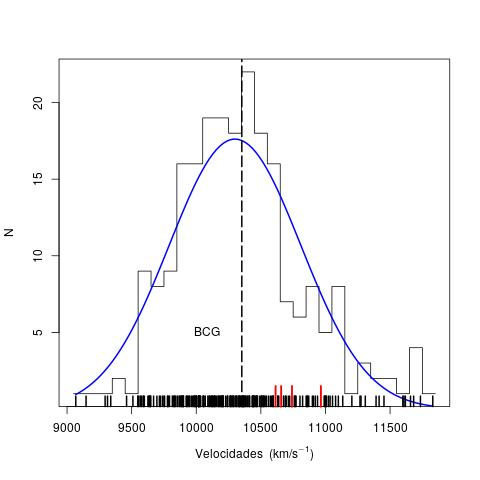
\includegraphics[scale=.23]{resultados/dist8}}
    \caption{Histograma Distribuição de Velocidade e Análise de \textit{gaps} Aglomerados 06, 07 e 08.}
  \end{figure}
\end{frame}

\begin{frame}{\textbf{Resultados Preliminares}}
  \begin{figure}[!htbp]
    \centering
    \subfloat{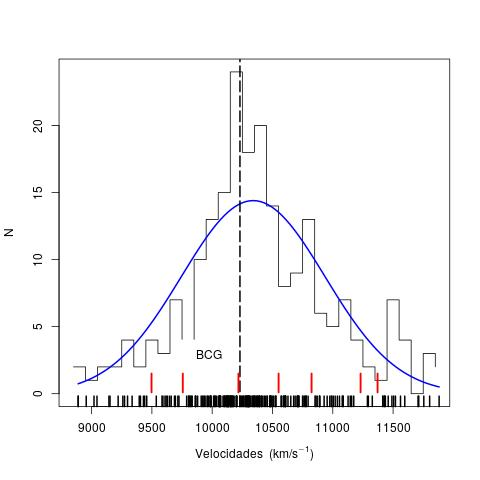
\includegraphics[scale=.23]{resultados/dist9}}
    \subfloat{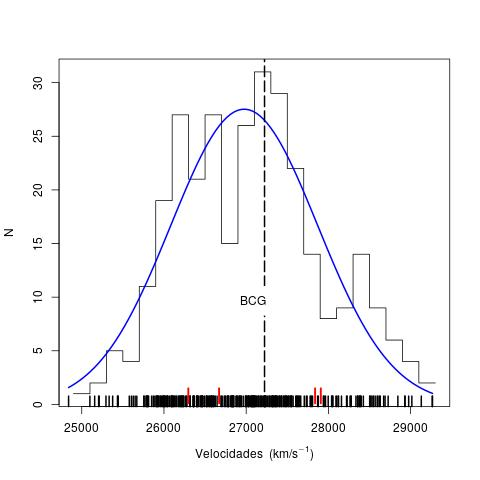
\includegraphics[scale=.23]{resultados/dist10}}
    \subfloat{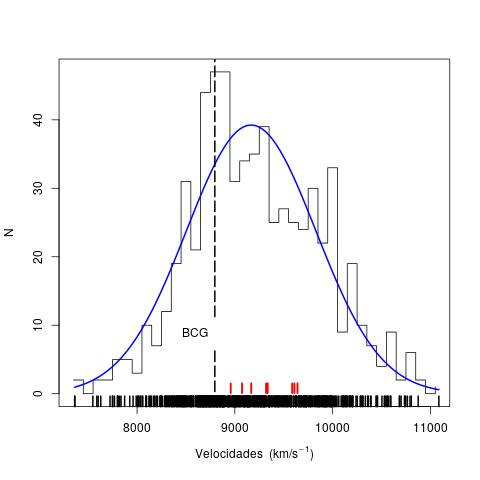
\includegraphics[scale=.23]{resultados/dist11}}
    \caption{Histograma Distribuição de Velocidade e Análise de \textit{gaps} Aglomerados 09, 10 e 11.}
  \end{figure}
\end{frame}

\begin{frame}{\textbf{Resultados Preliminares}}
  \begin{figure}[!htbp]
    \centering
    \subfloat{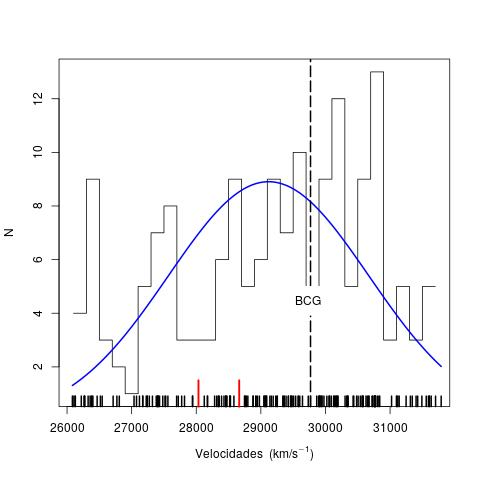
\includegraphics[scale=.23]{resultados/dist12}}
    \subfloat{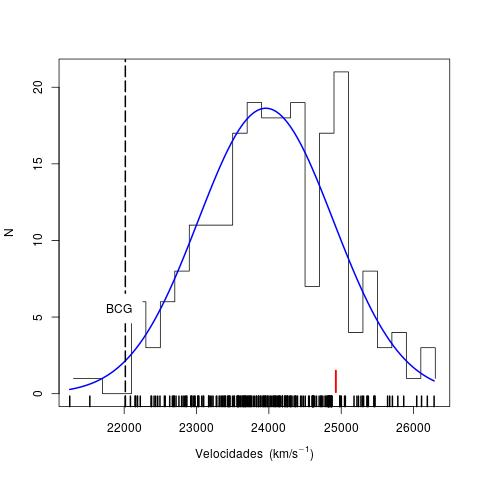
\includegraphics[scale=.23]{resultados/dist13}}
    \subfloat{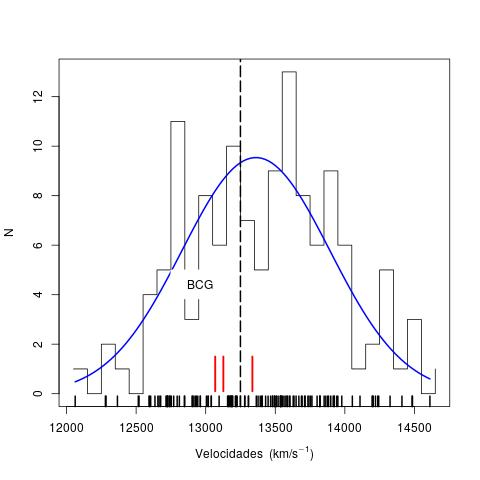
\includegraphics[scale=.23]{resultados/dist14}}
    \caption{Histograma Distribuição de Velocidade e Análise de \textit{gaps} Aglomerados 12, 13 e 14.}
  \end{figure}
\end{frame}

\begin{frame}{\textbf{Resultados Preliminares}}
  \begin{figure}[!htbp]
    \centering
    \subfloat{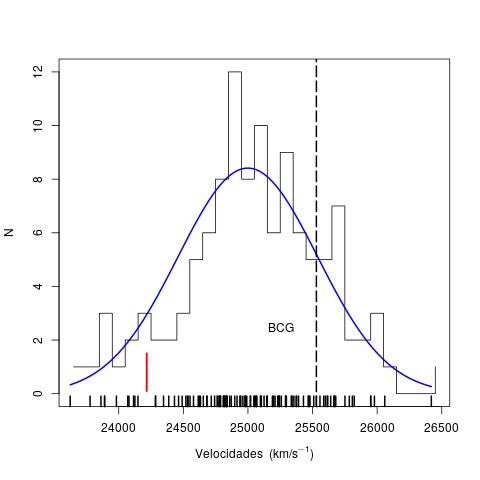
\includegraphics[scale=.23]{resultados/dist15}}
    \subfloat{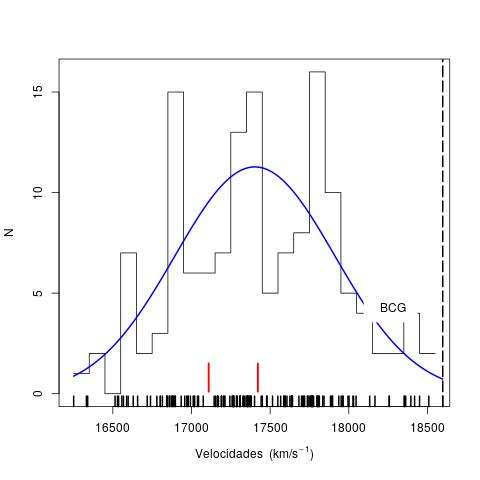
\includegraphics[scale=.23]{resultados/dist16}}
    \subfloat{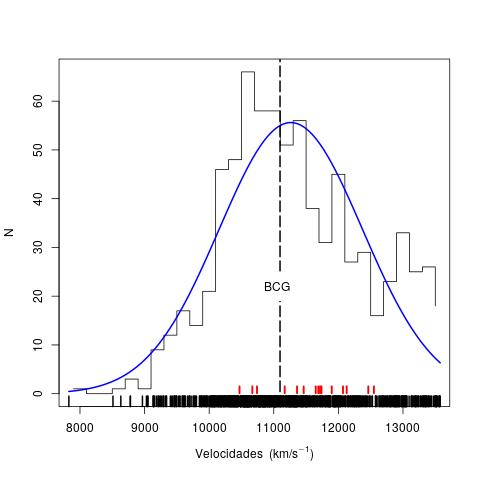
\includegraphics[scale=.23]{resultados/dist17}}
    \caption{Histograma Distribuição de Velocidade e Análise de \textit{gaps} Aglomerados 15, 16 e 17.}
  \end{figure}
\end{frame}

\begin{frame}{\textbf{Resultados Preliminares}}
  \begin{figure}[!htbp]
    \centering
    \subfloat{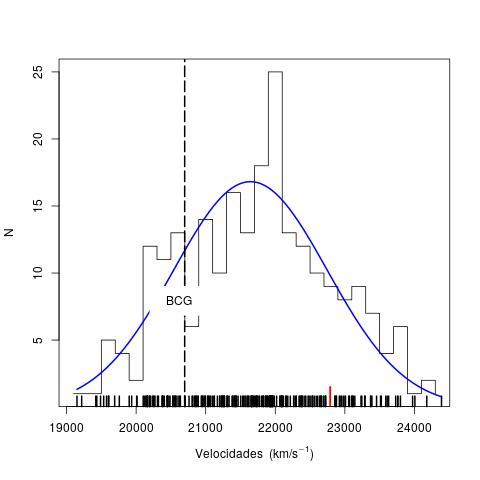
\includegraphics[scale=.23]{resultados/dist18}}
    \subfloat{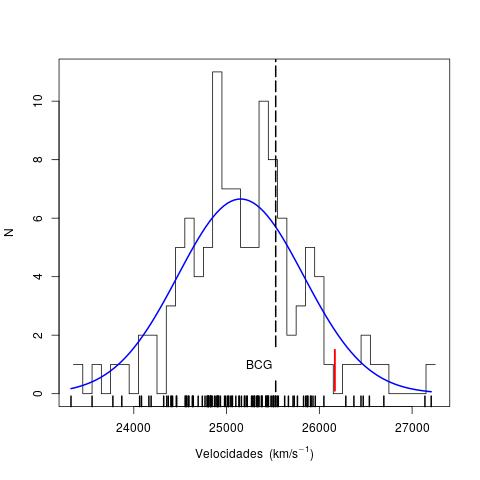
\includegraphics[scale=.23]{resultados/dist19}}
    \subfloat{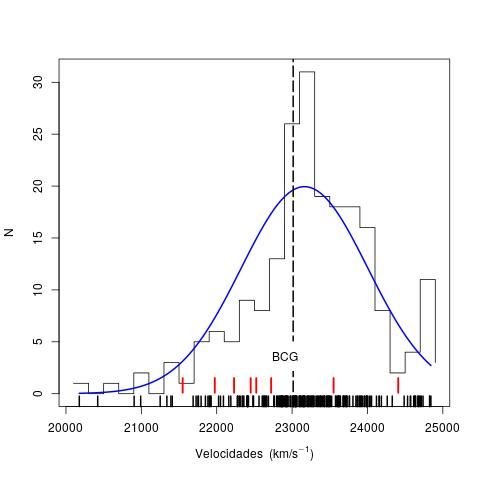
\includegraphics[scale=.23]{resultados/dist20}}
    \caption{Histograma Distribuição de Velocidade e Análise de \textit{gaps} Aglomerados 18, 19 e 20.}
  \end{figure}
\end{frame}


\begin{frame}{\textbf{Resultados Preliminares}}
  \begin{figure}[!htbp]
    \centering
    \subfloat{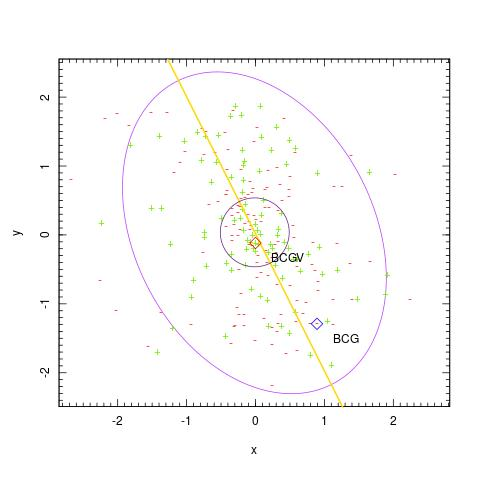
\includegraphics[scale=.3]{resultados/eixo1}}
    \subfloat{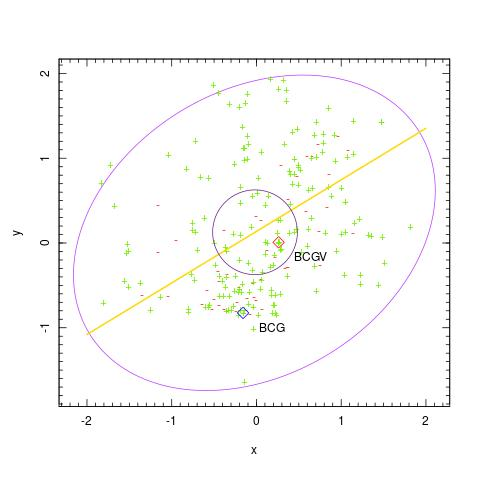
\includegraphics[scale=.3]{resultados/eixo2}}
    \caption{Histograma Distribuição de Velocidade e Análise de Gaps Aglomerados 01 e 02.}
  \end{figure}
\end{frame}

\begin{frame}{\textbf{Resultados Preliminares}}
  \begin{figure}[!htbp]
    \centering
    \subfloat{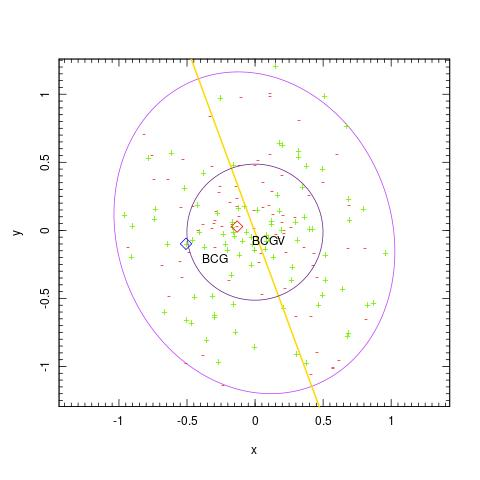
\includegraphics[scale=.23]{resultados/eixo3}}
    \subfloat{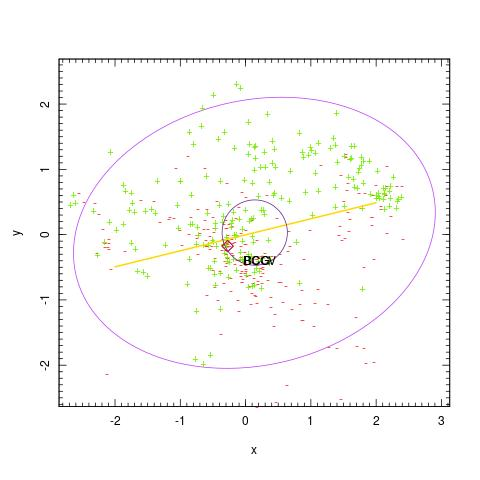
\includegraphics[scale=.23]{resultados/eixo4}}
    \subfloat{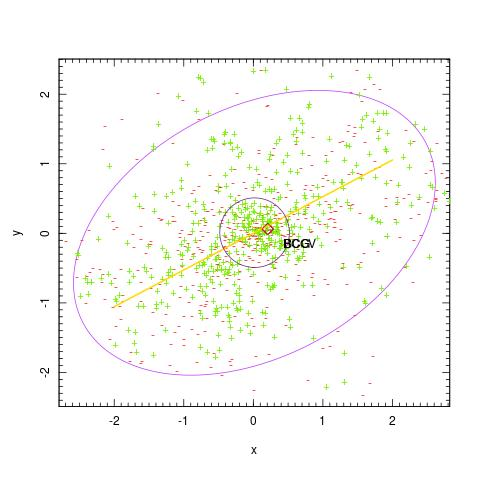
\includegraphics[scale=.23]{resultados/eixo5}}
    \caption{Histograma Distribuição de Velocidade e Análise de Gaps Aglomerados 03, 04 e 05.}
  \end{figure}
\end{frame}

\begin{frame}{\textbf{Resultados Preliminares}}
  \begin{figure}[!htbp]
    \centering
    \subfloat{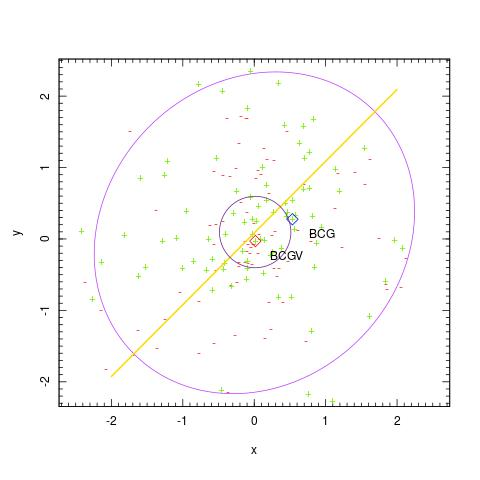
\includegraphics[scale=.23]{resultados/eixo6}}
    \subfloat{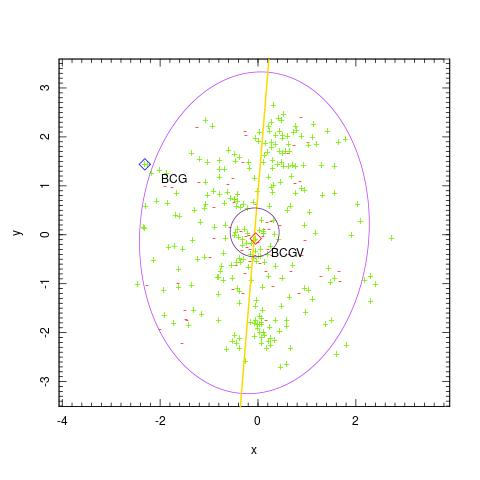
\includegraphics[scale=.23]{resultados/eixo7}}
    \subfloat{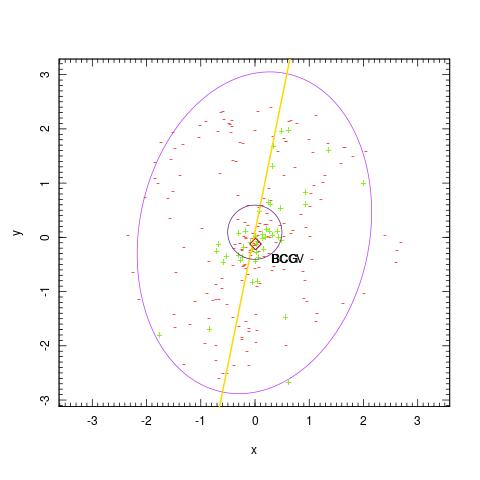
\includegraphics[scale=.23]{resultados/eixo8}}
    \caption{Histograma Distribuição de Velocidade e Análise de Gaps Aglomerados 06, 07 e 08.}
  \end{figure}
\end{frame}

\begin{frame}{\textbf{Resultados Preliminares}}
  \begin{figure}[!htbp]
    \centering
    \subfloat{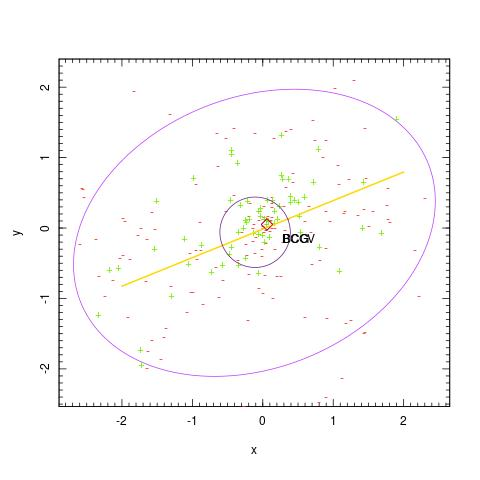
\includegraphics[scale=.23]{resultados/eixo9}}
    \subfloat{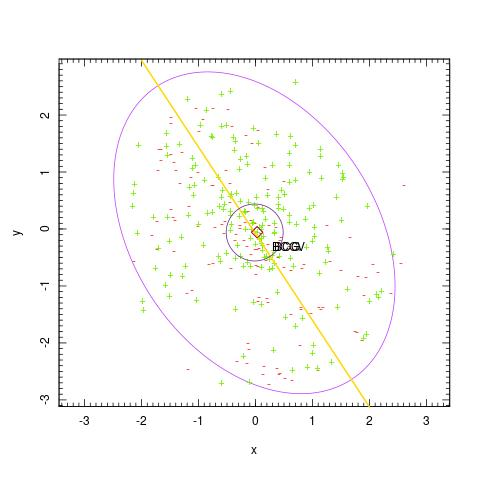
\includegraphics[scale=.23]{resultados/eixo10}}
    \subfloat{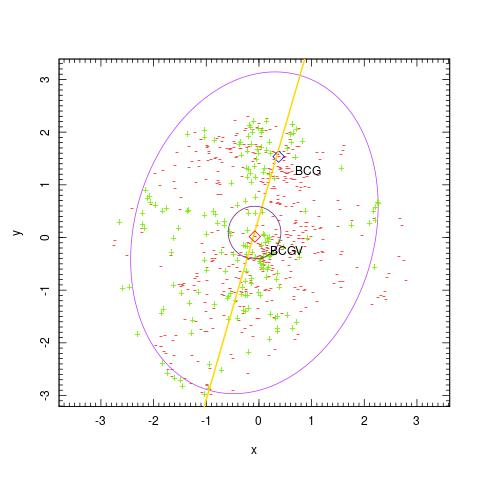
\includegraphics[scale=.23]{resultados/eixo11}}
    \caption{Histograma Distribuição de Velocidade e Análise de Gaps Aglomerados 09, 10 e 11.}
  \end{figure}
\end{frame}

\begin{frame}{\textbf{Resultados Preliminares}}
  \begin{figure}[!htbp]
    \centering
    \subfloat{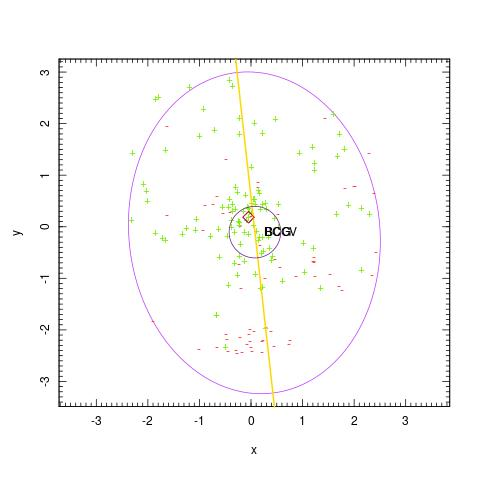
\includegraphics[scale=.23]{resultados/eixo12}}
    \subfloat{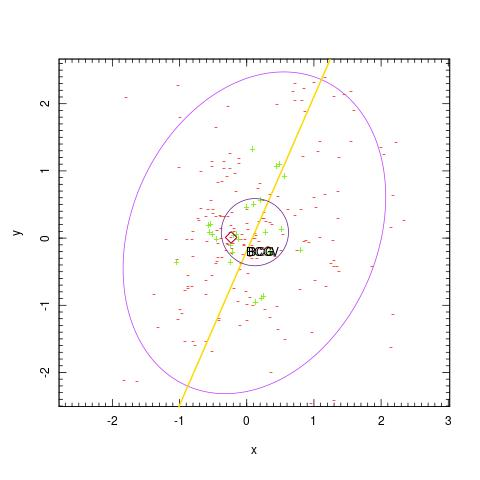
\includegraphics[scale=.23]{resultados/eixo13}}
    \subfloat{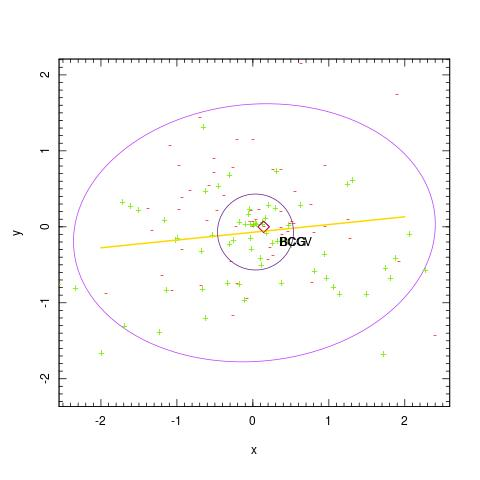
\includegraphics[scale=.23]{resultados/eixo14}}
    \caption{Histograma Distribuição de Velocidade e Análise de Gaps Aglomerados 12, 13 e 14.}
  \end{figure}
\end{frame}

\begin{frame}{\textbf{Resultados Preliminares}}
  \begin{figure}[!htbp]
    \centering
    \subfloat{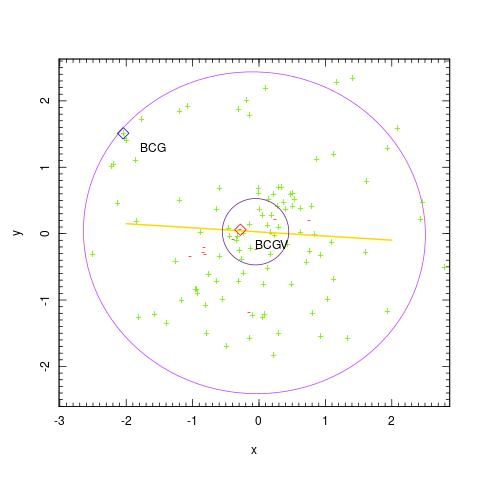
\includegraphics[scale=.23]{resultados/eixo15}}
    \subfloat{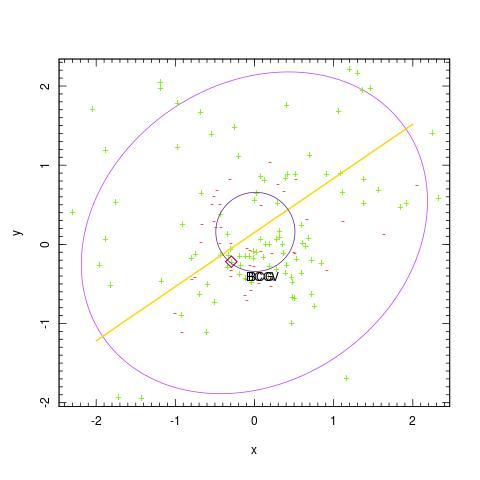
\includegraphics[scale=.23]{resultados/eixo16}}
    \subfloat{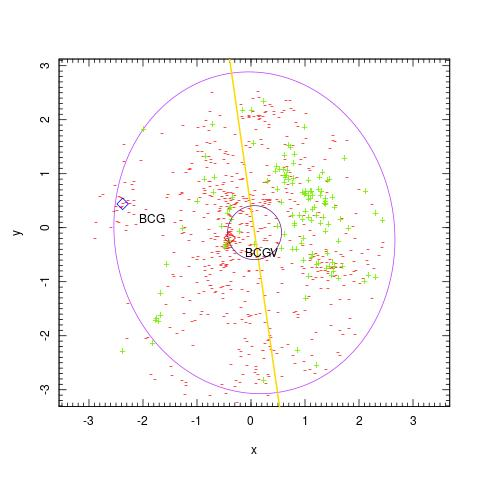
\includegraphics[scale=.23]{resultados/eixo17}}
    \caption{Histograma Distribuição de Velocidade e Análise de Gaps Aglomerados 15, 16 e 17.}
  \end{figure}
\end{frame}

\begin{frame}{\textbf{Resultados Preliminares}}
  \begin{figure}[!htbp]
    \centering
    \subfloat{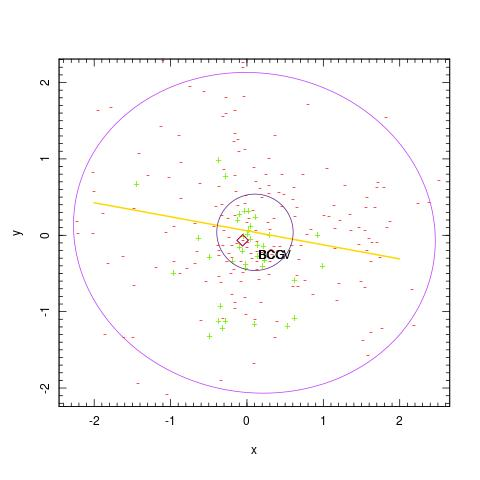
\includegraphics[scale=.23]{resultados/eixo18}}
    \subfloat{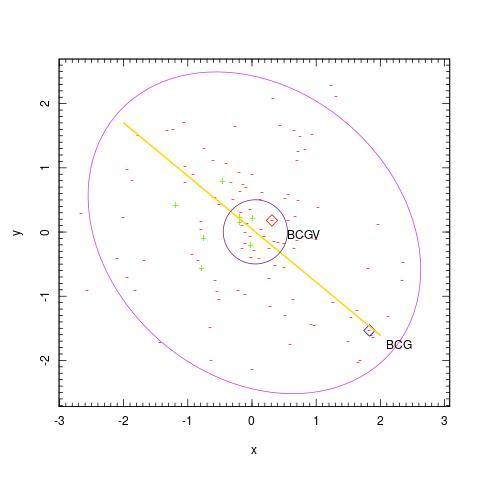
\includegraphics[scale=.23]{resultados/eixo19}}
    \subfloat{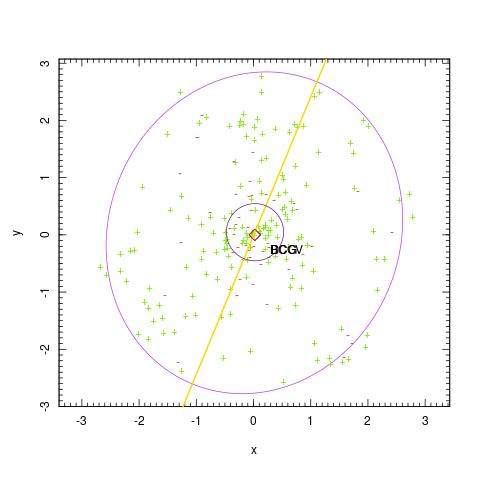
\includegraphics[scale=.23]{resultados/eixo20}}
    \caption{Histograma Distribuição de Velocidade e Análise de Gaps Aglomerados 18, 19 e 20.}
  \end{figure}
\end{frame}

\begin{frame}{\textbf{Resultados Preliminares}}
\begin{table}[!htbp]
\caption{Teste Cramér e Hotelling em todos os pontos.}
\vspace{10pt}
\centering{}
\resizebox{.55\textwidth}{!}{
\begin{tabular*}{\textwidth}{@{\extracolsep{\fill}}ccc}     
\hline
\textbf{Aglomerado} & \textbf{Teste de Cramér \textit{p-value}} & \textbf{Teste de Hotelling \textit{p-value}} \\
\hline
 01 & 0.5064 & 0.6160 \\  
%\hline
 02 &{\color{red}  0.0059} & {\color{red} 0.0078}\\ 
%\hline
 03 & 0.3376  & 0.5612   \\ 
%\hline
 04 & {\color{red}0.0009} & {\color{red}$<$0.0001} \\ 
%\hline
 05 &  0.1018 &  {\color{red}0.0723} \\ 
%\hline
 06 &  0.2357 &   0.8041 \\ 
%\hline
 07 & 0.0519 &   0.6347 \\ 
%\hline
 08 & {\color{red}0.0069}  &  0.0807 \\ 
%\hline
 09 & {\color{red}0.0279} &  {\color{red}0.0373}  \\ 
%\hline
 10 & {\color{red}0.0009} & {\color{red}0.0258}   \\ 
%\hline
 11 &  {\color{red}0.0049} & 0.9006  \\ 
%\hline
 12 & {\color{red}$<$0.0001} & {\color{red}$<$0.0001}\\ 
%\hline
 13 &  0.1148  &   0.1516   \\ 
%\hline
 14 & {\color{red}0.0289} & {\color{red}0.0054}  \\ 
%\hline
 15 & 0.1148 & 0.5745 \\ 
%\hline
 16 & 0.0629 &  0.5182 \\ 
%\hline
 17 & $<$0.0001 &  $<$0.0001\\ 
%\hline
 18 & {\color{red}$<$0.0001} &  {\color{red}0.0075}\\ 
%\hline
 19 & 0.0939 &   0.4063\\ 
%\hline
 20 &  0.1018 & 0.9038 \\
\hline
\label{table1}
\end{tabular*}
}
\end{table}
\end{frame}

\begin{frame}{\textbf{Resultados Preliminares}}
\begin{table}[!htbp]
\caption{Teste Cramér e Hotelling pontos acima do eixo.}
\vspace{10pt}
\centering{}
\resizebox{.55\textwidth}{!}{
\begin{tabular*}{\textwidth}{@{\extracolsep{\fill}}ccc}     
\hline
\textbf{Aglomerado} & \textbf{Teste de Cramér \textit{p-value}} & \textbf{Teste de Hotelling \textit{p-value}} \\
\hline
 01 & 0.7772 & 0.8718 \\  
%\hline
 02 &  0.0959 &  {\color{red}0.0069} \\ 
%\hline
 03 & 0.6623 & 0.2025  \\ 
%\hline
 04 & {\color{red}0.0009} & {\color{red}$<$0.0001} \\ 
%\hline
 05 &  {\color{red}0.0319} & {\color{red}0.0483}  \\ 
%\hline
 06 &  0.4575 &   0.2650 \\ 
%\hline
 07 & 0.5894&  0.5880\\ 
%\hline
 08 &  {\color{red}0.0049}  &  0.4446 \\ 
%\hline
 09 &  {\color{red}0.0389}  &  0.2302 \\ 
%\hline
 10 & {\color{red}0.0029} & {\color{red}0.0067 } \\ 
%\hline
 11 &  0.3386 &  {\color{red}0.0031} \\ 
%\hline
 12 &{\color{red} $<$0.0001 }& {\color{red}$<$0.0001}\\ 
%\hline
 13 &  0.1518  &   0.6982  \\ 
%\hline
 14 &  0.4795 & 0.0054  \\ 
%\hline
 15 & 0.3406  & 0.5745 \\ 
%\hline
 16 & {\color{red}0.0059} &  0.5182 \\ 
%\hline
 17 & {\color{red}$<$0.0001} & {\color{red}$<$0.0001} \\ 
%\hline
 18 & {\color{red}0.0169} &  {\color{red}0.0075}\\ 
%\hline
 19 & 0.2817 &   0.4063\\ 
%\hline
 20 &  0.0699 & 0.3173 \\
\hline
\label{table2}
\end{tabular*}
}
\end{table}
\end{frame}


\begin{frame}{\textbf{Resultados Preliminares}}
  \begin{table}[!htbp]
\caption{Teste Cramér e Hotelling pontos abaixo do eixo.}
\vspace{10pt}
\centering{}
\resizebox{.55\textwidth}{!}{
\begin{tabular*}{\textwidth}{@{\extracolsep{\fill}}ccc}     
\hline
\textbf{Aglomerado} & \textbf{Teste de Cramér \textit{p-value}} & \textbf{Teste de Hotelling \textit{p-value}} \\
\hline
 01 & 0.3836 & 0.7469 \\  
%\hline
 02 &{\color{red} 0.0299} &  0.0916 \\ 
%\hline
 03 & 0.0759  & 0.1299  \\ 
%\hline
 04 & {\color{red}$<$0.0001} & {\color{red}$<$0.0001} \\ 
%\hline
 05 &  0.1018 & {\color{red}0.0483}  \\ 
%\hline
 06 &  0.2357 &   0.2650 \\ 
%\hline
 07 & 0.0519 &  0.5880\\ 
%\hline
 08 & {\color{red}0.0069}  &  0.4446 \\ 
%\hline
 09 & {\color{red}0.0279} &  0.2302 \\ 
%\hline
 10 & {\color{red}0.0009} & {\color{red}0.0067}  \\ 
%\hline
 11 &  {\color{red}0.0049} &  {\color{red}0.0031} \\ 
%\hline
 12 & {\color{red}$<$0.0001} & {\color{red}$<$0.0001}\\ 
%\hline
 13 &  0.1148  &   0.6982  \\ 
%\hline
 14 & {\color{red}0.0289} & {\color{red}0.0054}  \\ 
%\hline
 15 & 0.1148 & 0.5745 \\ 
%\hline
 16 & 0.0629 &  0.5182 \\ 
%\hline
 17 & {\color{red}$<$0.0001} &  {\color{red}$<$0.0001}\\ 
%\hline
 18 & {\color{red}$<$0.0001} &  {\color{red}0.0075}\\ 
%\hline
 19 & 0.0939 &   0.4063\\ 
%\hline
 20 &  0.1018 & 0.9038 \\
\hline
\label{table3}
\end{tabular*}
}
\end{table}
\end{frame}

\begin{frame}{\textbf{Aglomerados com evidência de algum grau de rotação}}
  \begin{itemize}
    \item Aglomerados: 02, {\color{red}04}, 05, 08, 09, {\color{red}10}, 11, {\color{red}12}, 14, 16, 17, {\color{red}18}
  \end{itemize}
  \begin{block}{Velocidade de Rotação}
  \begin{equation}
    \omega= \Delta V/R 
  \end{equation}
   \textbf{Unidades:} $V = km/s^{-1}  \hspace{2 ex} e \hspace{2 ex} R = Mpc$
  \end{block}
\end{frame}


\begin{frame}
  \begin{figure}[!htbp] %h or !htbp
  \vspace{-2pt}
  \begin{center}
  \subfloat{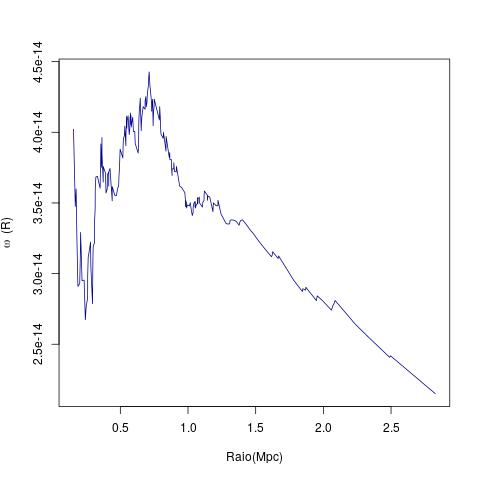
\includegraphics[scale=.23]{resultados/perfil2}}%
  \subfloat{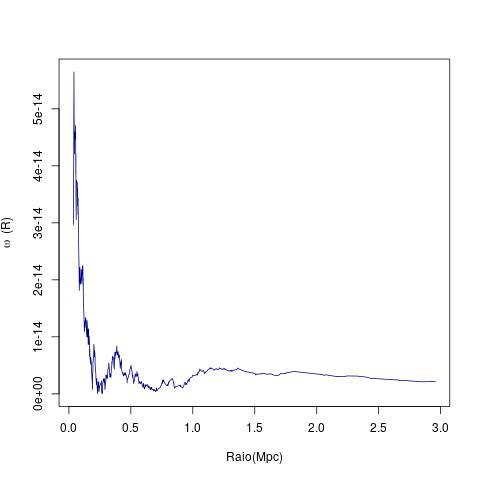
\includegraphics[scale=.23]{resultados/perfil4}}
  \subfloat{\includegraphics[scale=.23]{resultados/perfil5}}
  \caption{Perfil da velocidade de rotação Aglomerados 02, 04 e 05.}
  \label{fig6}%
  \end{center}
  \end{figure}
\end{frame}

\begin{frame}
  \begin{figure}[!htbp] %h or !htbp
  \vspace{-2pt}
  \begin{center}
  \subfloat{\includegraphics[scale=.23]{resultados/perfil8}}
  \subfloat{\includegraphics[scale=.23]{resultados/perfil9}}
  \subfloat{\includegraphics[scale=.23]{resultados/perfil10}}
  \caption{Perfil da velocidade de rotação Aglomerados 08, 09 e 10.}
  \label{fig6}%
  \end{center}
  \end{figure}
\end{frame}

\begin{frame}
  \begin{figure}[!htbp] %h or !htbp
  \vspace{-2pt}
  \begin{center}
    \subfloat{\includegraphics[scale=.23]{resultados/perfil11}}%
    \subfloat{\includegraphics[scale=.23]{resultados/perfil12}}
    \subfloat{\includegraphics[scale=.23]{resultados/perfil14}}
    \caption{Perfil da velocidade de rotação Aglomerados 11, 12 e 14.}
    \label{fig6}%
  \end{center}
  \end{figure}
\end{frame}

\begin{frame}
  \begin{figure}[!htbp] %h or !htbp
  \vspace{-2pt}
  \begin{center}
    \subfloat{\includegraphics[scale=.23]{resultados/perfil16}}
    \subfloat{\includegraphics[scale=.23]{resultados/perfil17}}%
    \subfloat{\includegraphics[scale=.23]{resultados/perfil18}}
    \caption{Perfil da velocidade de rotação Aglomerados 16, 17 e 18.}
    \label{fig6}%
  \end{center}
  \end{figure}
\end{frame}

\begin{frame}
	 \begin{figure}[!htbp] %h or !htbp
  \vspace{-2pt}
  \begin{center}
    \includegraphics[scale=.8]{resultados/rotacao.png}
    \caption{Velocidade rotacional identificada no Aglomerado 02.}
    \label{rotate}%
  \end{center}
  \end{figure}
  \begin{center}
  	9.37 Manos
  \end{center}
\end{frame}

\section{Perspectivas}
\begin{frame}{Perspectivas}
  \begin{itemize}
    \item Pretendemos repetir o cálculo usando a mediana da distribuição, como no método de Tovmassian (2015) e a definição de substruturas, quando existirem, para a divisão de aglomerados, ao invés do uso do {\it gap} principal.
    \item Implementar e realizar uma comparação de nosso método com aquele de Hwang \& Lee (2007).
    \item Aplicar nosso programa a um conjunto maior de dados, aproximadamente 500 aglomerados do SDSS, definida originalmente por Miller et al. (2005) com dados do SDSS-DR2 e redefinida aqui com dados do SDSS-DR12.
    \item Cálculo da massa do aglomerado com correção de rotação.
  \end{itemize}
\end{frame}


\begin{frame}{Perspectivas}
\begin{itemize}
  \item Cronograma para os próximos meses
\end{itemize}
\begin{table}[]
\resizebox{1.0  \textwidth}{!}{
\begin{tabular}{|l|c|c|c|c|c|c|c|c|}
\hline
\multicolumn{1}{|c|}{\textbf{Atividades}}        & \multicolumn{1}{l|}{\textbf{15/09}} & \multicolumn{1}{l|}{\textbf{30/09}} & \multicolumn{1}{l|}{\textbf{15/10}} & \multicolumn{1}{l|}{\textbf{31/10}} & \multicolumn{1}{l|}{\textbf{15/11}} & \multicolumn{1}{l|}{\textbf{30/11}} & \multicolumn{1}{l|}{\textbf{15/12}} & \multicolumn{1}{l|}{\textbf{31/12}} \\ \hline
Implementação do método de Hwang \& Lee (2007)   & x                                   & x                                   & x                                   &                                     &                                     &                                     &                                     &                                     \\ \hline
Implementação das alternativas ao cálculo de gap &                                    &             x                        &                x                     &                                     &                                     &                                     &                                     &                                     \\ \hline
Aplicação dos métodos em uma amostra maior       &                                     &                                     &                                     & x                                   & x                                   &                                     &                                     &                                     \\ \hline
Análise dos resultados                           &                                     &                                     &                                     &                                     &                                     & x                                   &                                     &                                     \\ \hline
Escrita da dissertação                           & x                                   & x                                   & x                                   & x                                   & x                                   & x                                   & x                                   & x                                   \\ \hline
\end{tabular}
}
\end{table}
\end{frame}

\section{Referências}
\begin{frame}{Referências}
  \begin{thebibliography}{9}
  \fontsize{8}{0}\selectfont
  \bibitem[Chluba \& Mannheim, 2002]{chluba2002}
  Chluba, J.; Mannheim,. Kinetic Sunyaev-Zeldovich effect from galaxy cluster rotation. MNRAS, v. 396, p. 419 -
  427, Agosto 2002.

  \bibitem[Beers et~al., 1990]{Beers1990}
  Beers, T. C., Flynn K., Gebhardt K., 1990, AJ, 100, 32. 

  \bibitem[de Oliveira et~al., 2004]{deOliveira2004}
  de Oliveira, F.; Viegas, S. M. M. Descobrindo o Universo. São Paulo: Edusp, v. 56, 2004.

  \bibitem[Fang et~al, 2008]{Fang2008}
  Fang, T.; Humphrey, P. J.; Buote, D. A. Rotation and Turbulence of the Hot ICM in Galaxy Clusters. MNRAS,
  v. 691, p. 1648-1659, Agosto 2008.

  \bibitem[Friaça et~al, 2008]{Friaca2008}
  Friaça, A. C. S. et al. Astronomia: Uma Visão Geral do Universo. 2a. ed. São Paulo: EDUSP, v. 28, 2008.

  \end{thebibliography}
\end{frame}

\begin{frame}{Referências}
  \begin{thebibliography}{9}
  \fontsize{8}{0}\selectfont
  \bibitem[Hamden et~al, 2010]{Hamden2010}
  Hamden, E. T. et al. Measuring Transverse Motions for Nearby Galaxy Clusters. MNRAS, Maio 2010.

  \bibitem[Hwang \& Lee, 2007]{Hwang2007}
  HWANG, Ho Seong; LEE, Myung Gyoon. Searching for rotating galaxy clusters in SDSS and 2dFGRS. {The Astrophysical Journal}, v. 662, n. 1, p. 236, 2007.

  \bibitem[Kalinkov et~al, 2005]{Kalinkov2005}
  Kalinkov, M. et al. Rotation of the cluster of galaxies A2107. MNRAS, v. 359 , p. 1491-1497, Maio 2005.

  \bibitem[Manolopoulou et~al., 2008]{Manolopoulou2016}
  Manolopoulou, M.; Plionis, M. Galaxy cluster's rotation. MNRAS, v. 465 , p. 2616-2633, Abril 2016.

  \bibitem[Miller et~al., 2005]{Miller2005}
  Miller et al. 2005, Article (PDF Available) in the Astronomical Journal 130(3):198, December 2007. 

  \bibitem[Nascimento, 2012]{Nascimento2012}
  Nascimento, R. S. Estudo da dinâmica de pares de aglomerados de galáxias. Dissertação (Programa de Pós-
  graduação em Física) - UESC. Ilhéus, p. 91. 2012.
  \end{thebibliography}
\end{frame}

\begin{frame}{Referências}
  \begin{thebibliography}{9}
  \fontsize{8}{0}\selectfont
  \bibitem[Ribeiro et~al, 2011]{Ribeiro2011}
  Ribeiro A. L. B., Lopes P. A. A., Trevisan M., 2011, MNRAS, 413, L81.

  \bibitem[Rembold, 2011]{Rembold2011}
  Rembold, B. Tópicos especiais em física: Astronomia. Ilhéus: UAB /UESC, v. 4, 2011. 384 p.

  \bibitem[Sampaio, 2013]{Sampaio2013}
  Sampaio, F. S. Estudo da Distribuição de velocidades em aglomerados de galáxias - Testes de Não Rejeitaidade e
  metanálise de Fisher. Dissertação (Programa de Pós-Graduação em Física) - UESC. Ilhéus, p. 51. 2013.

  \bibitem[Tovmassian, 2015]{Tovmassian2015}
  Tovmassian, H. M. The rotation of Galaxy Clusters. Astrophysics, v. 58, p. 353-363, Setembro 2015.

  \bibitem[Velásquez, 2007]{Velasquez2017}
  Velásquez, C. A. M. Estimativa de Parâmetros Cosmológicos usando Aglomerados de Galáxias. Dissertação
  (Programa de Pós-Graduação em Astronomia) - UFRJ. Rio de Janeiro, p. 74. 2007.

  \bibitem[Yahil et~al., 1997]{Yahil1997}
  Yahil, A \& Vidal, N. V The Velocity Distribution Of Galaxies In Clusters Ap. J. N 214, 347-350, 1997.
  \end{thebibliography}
\end{frame}

\end{document}